%%
%% Beuth Hochschule für Technik --  
%%
%% Kapitel 3 - Android App
%%
%%	

\chapter{Android App}
\section{Android}
Das Betriebssystem ist komplett in der Sprache Java programmiert worden. Dabei handelt es sich um ein Open Source Betriebssystem, welches von der Firma Google entwickelt worden ist. Kern des Betriebssystems ist ein angepasster Linux-Kernel 2.6. 
\subsection{Struktur und Aufbau der App}

\begin{figure}[h]
  \begin{center}
    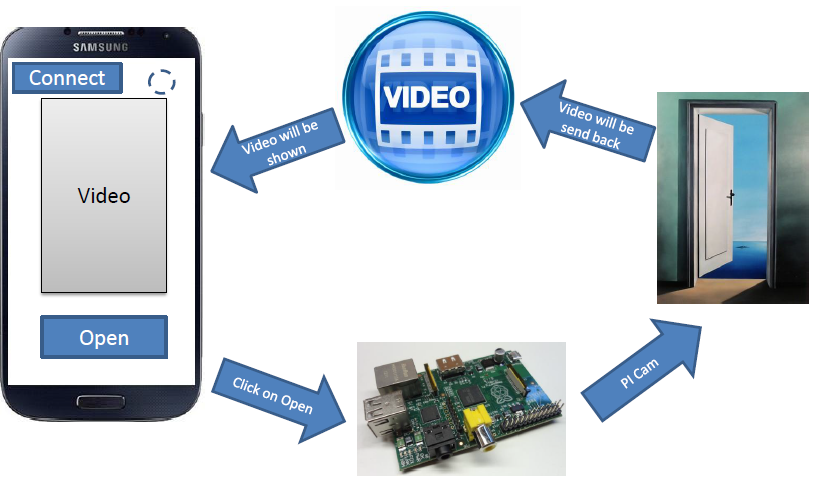
\includegraphics[scale=0.3]{process.png}
  		  \caption{Prozess der App}
     \label{fig.Prozess}
  \end{center}
\end{figure}

Die Türspion-App (Spyhole) besteht aus verschiedenen Ebenen sogenannten Activities. Jede Activity stellt eine bestimmte Benutzerschnittstelle dar, wie zum Beispiel der Login oder die Registrierung.

Dabei wird beim Start der ein Splash-Screen angezeigt, die den Benutzer Willkommen heißt und nach einer kurzen Zeit wird, der Nutzer auf die Übersichtsseite weitergeleitet.

%%%%%%%%%%%%%%%%%%%%%%%%%%%%%%%%%%%%%%%%%%%%%%%%%%%%%%%%%%%%%%%%%%
\subsection{Login}
Der Login sollte als Sicherheit in die App eingebaut werden, die Implementierung dieses Teils konnte leider nicht fertiggestellt werden, da bestimmte technische Probleme auftraten, die in der Zeit nicht gelöst werden konnten. Im Folgenden soll aber dennoch die Vorgehensweise beschrieben werden und welche Technologien verwendet worden sind.
\subsubsection{Registrierung}
\begin{figure}[h]
  \begin{center}
    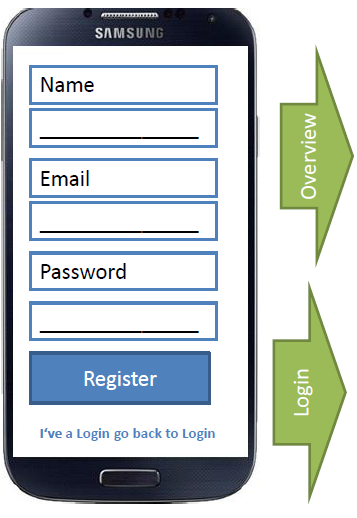
\includegraphics[scale=0.3]{register.png}
  		  \caption{Registrierung}
     \label{fig.Prozess}
  \end{center}
\end{figure}
Um sich überhaupt einloggen zu können muss sich der Benutzer erst einmal registrieren. Dabei muss der Nutzer seine 
\begin{itemize}
	\item{E-Mail}
	\item{Nutzername}
	\item{Passwort}
\end{itemize}
eingeben. Diese Daten werden alle in ein JSON-Objekt geschrieben und per POST-Methode an den Server gesendet. Auf dem Server wird in der Index.php erkannt, dass sich ein neuer Nutzer anmelden möchte dem entsprechend wird in einer Mehrfachauswahl (Switch-Case) ausgewertet und in einem weiteren PHP-Skript weiter bearbeitet. Schlussendlich werden die Daten in eine MySQL-Datenbank in die jeweiligen Spalten geschrieben. Das eingegebene Passwort beim Eintragen in die Datenbank verschlüsselt, dass mögliche Hacker die das Password nicht auslesen können. 
\subsubsection{Der eigentliche Login}
\begin{figure}[h]
  \begin{center}
    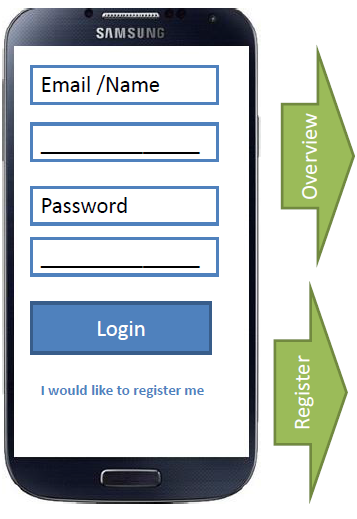
\includegraphics[scale=0.3]{login.png}
  		  \caption{Login}
     \label{fig.Prozess}
  \end{center}
\end{figure}

Beim Login verläuft der Vorgang wie bei der eben beschriebenen Registrierung, bloß in die andere Richtung. Dabei wird ein JSON-Objekt vom Server an das mobile Endgerät geschickt und in der App aufgeschlüsselt und interpretiert. Danach wird verglichen ob sich der Nutzer der sich gerade einloggen möchte schon eingetragen ist, wenn ja wird auf die nächste Activity weitergeleitet, ansonsten wird er zur Registrierung geführt und gebeten sich anzumelden.
\subsection{Control View}
\begin{figure}[h]
  \begin{center}
    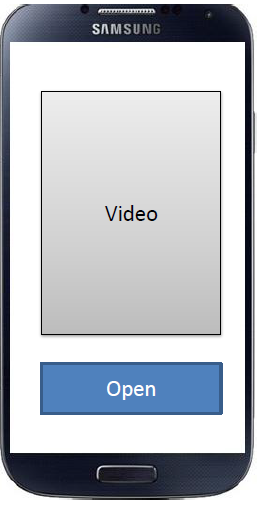
\includegraphics[scale=0.3]{controlcenter.png}
  		  \caption{Control View}
     \label{fig.Prozess}
  \end{center}
\end{figure}
\subsection{Datenbank}
\begin{figure}[h]
  \begin{center}
    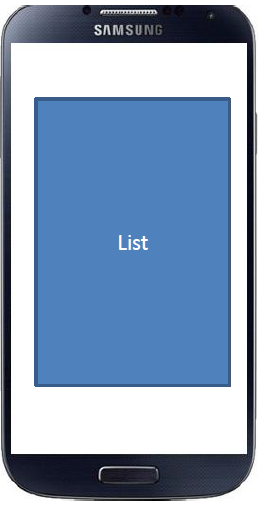
\includegraphics[scale=0.3]{database.png}
  		  \caption{Datenbank}
     \label{fig.Prozess}
  \end{center}
\end{figure}